% Himalayan expeditions -- SML project presentation (15 min + backup)
% Compile from this folder:  latexmk presentation.tex   (pdfLaTeX, settings in latexmkrc)
% All figures and numbers come from ../analysis.R and ../figures.R (figures/, results/results.txt).
% Figures are drawn at their on-slide size, so they are included without scaling.
\documentclass[aspectratio=169,10pt,t]{beamer}
\usepackage[T1]{fontenc}
\usepackage{lmodern}
\usepackage{booktabs}
\usepackage{array}
\usepackage{graphicx}
\usepackage{amsmath}
\usepackage{tikz}
\usepackage{appendixnumberbeamer}
\graphicspath{{../figures/}}

% ---- classic Beamer look --------------------------------------------------------------------
\usefonttheme[onlymath]{serif}                     % maths in Computer Modern
\definecolor{navy}{HTML}{1F3F73}
\setbeamercolor{structure}{fg=navy}
\setbeamercolor{normal text}{fg=black}
\setbeamercolor{frametitle}{fg=navy}
\setbeamercolor{title}{fg=navy}
\setbeamercolor{block title}{fg=navy,bg=navy!8}
\setbeamercolor{block body}{bg=navy!3}
\setbeamertemplate{blocks}[rounded][shadow=false]
\setbeamertemplate{navigation symbols}{}
\setbeamertemplate{itemize items}[circle]
\setbeamertemplate{enumerate items}[default]
\setbeamersize{text margin left=0.9cm, text margin right=0.9cm}
\setbeamerfont{frametitle}{size=\large,series=\bfseries}
\setbeamertemplate{frametitle}{%
  \vspace*{0.35em}\insertframetitle\par\vspace{-0.25em}{\color{black!25}\rule{\textwidth}{0.4pt}}\par\vspace{-0.6em}}
\setbeamertemplate{footline}{%
  \leavevmode\hbox to \paperwidth{\hfill\tiny\color{black!55}\insertframenumber\hspace{0.9cm}}\vspace{2.2mm}}

% captions: small, grey, one line where possible
\setbeamertemplate{caption}[numbered]
\setbeamertemplate{caption label separator}{: }
\setbeamerfont{caption}{size=\scriptsize}
\setbeamerfont{caption name}{series=\bfseries}
\setbeamercolor{caption}{fg=black!60}
\setbeamercolor{caption name}{fg=black!60}
\setlength{\abovecaptionskip}{2pt}
\setlength{\belowcaptionskip}{0pt}
\newcommand{\fig}[3][]{\begin{figure}\centering\includegraphics[#1]{#2}\caption{#3}\end{figure}}
% side-by-side panels: the visual sits in a box of fixed height, so captions (and anything
% below them) start at the same height in both columns.  \cell{env}{height}{content}{caption}
\newcommand{\cell}[4]{\begin{#1}\parbox[c][#2][c]{\linewidth}{\centering #3}\caption{#4}\end{#1}}

\begin{document}

% ---------------------------------------------------------------- title
\begin{frame}[plain]
\begin{tikzpicture}[remember picture, overlay]
  \begin{scope}
    \clip ([xshift=0.6\paperwidth]current page.north west) rectangle (current page.south east);
    \node at ([xshift=-0.2\paperwidth+2.5mm]current page.east) {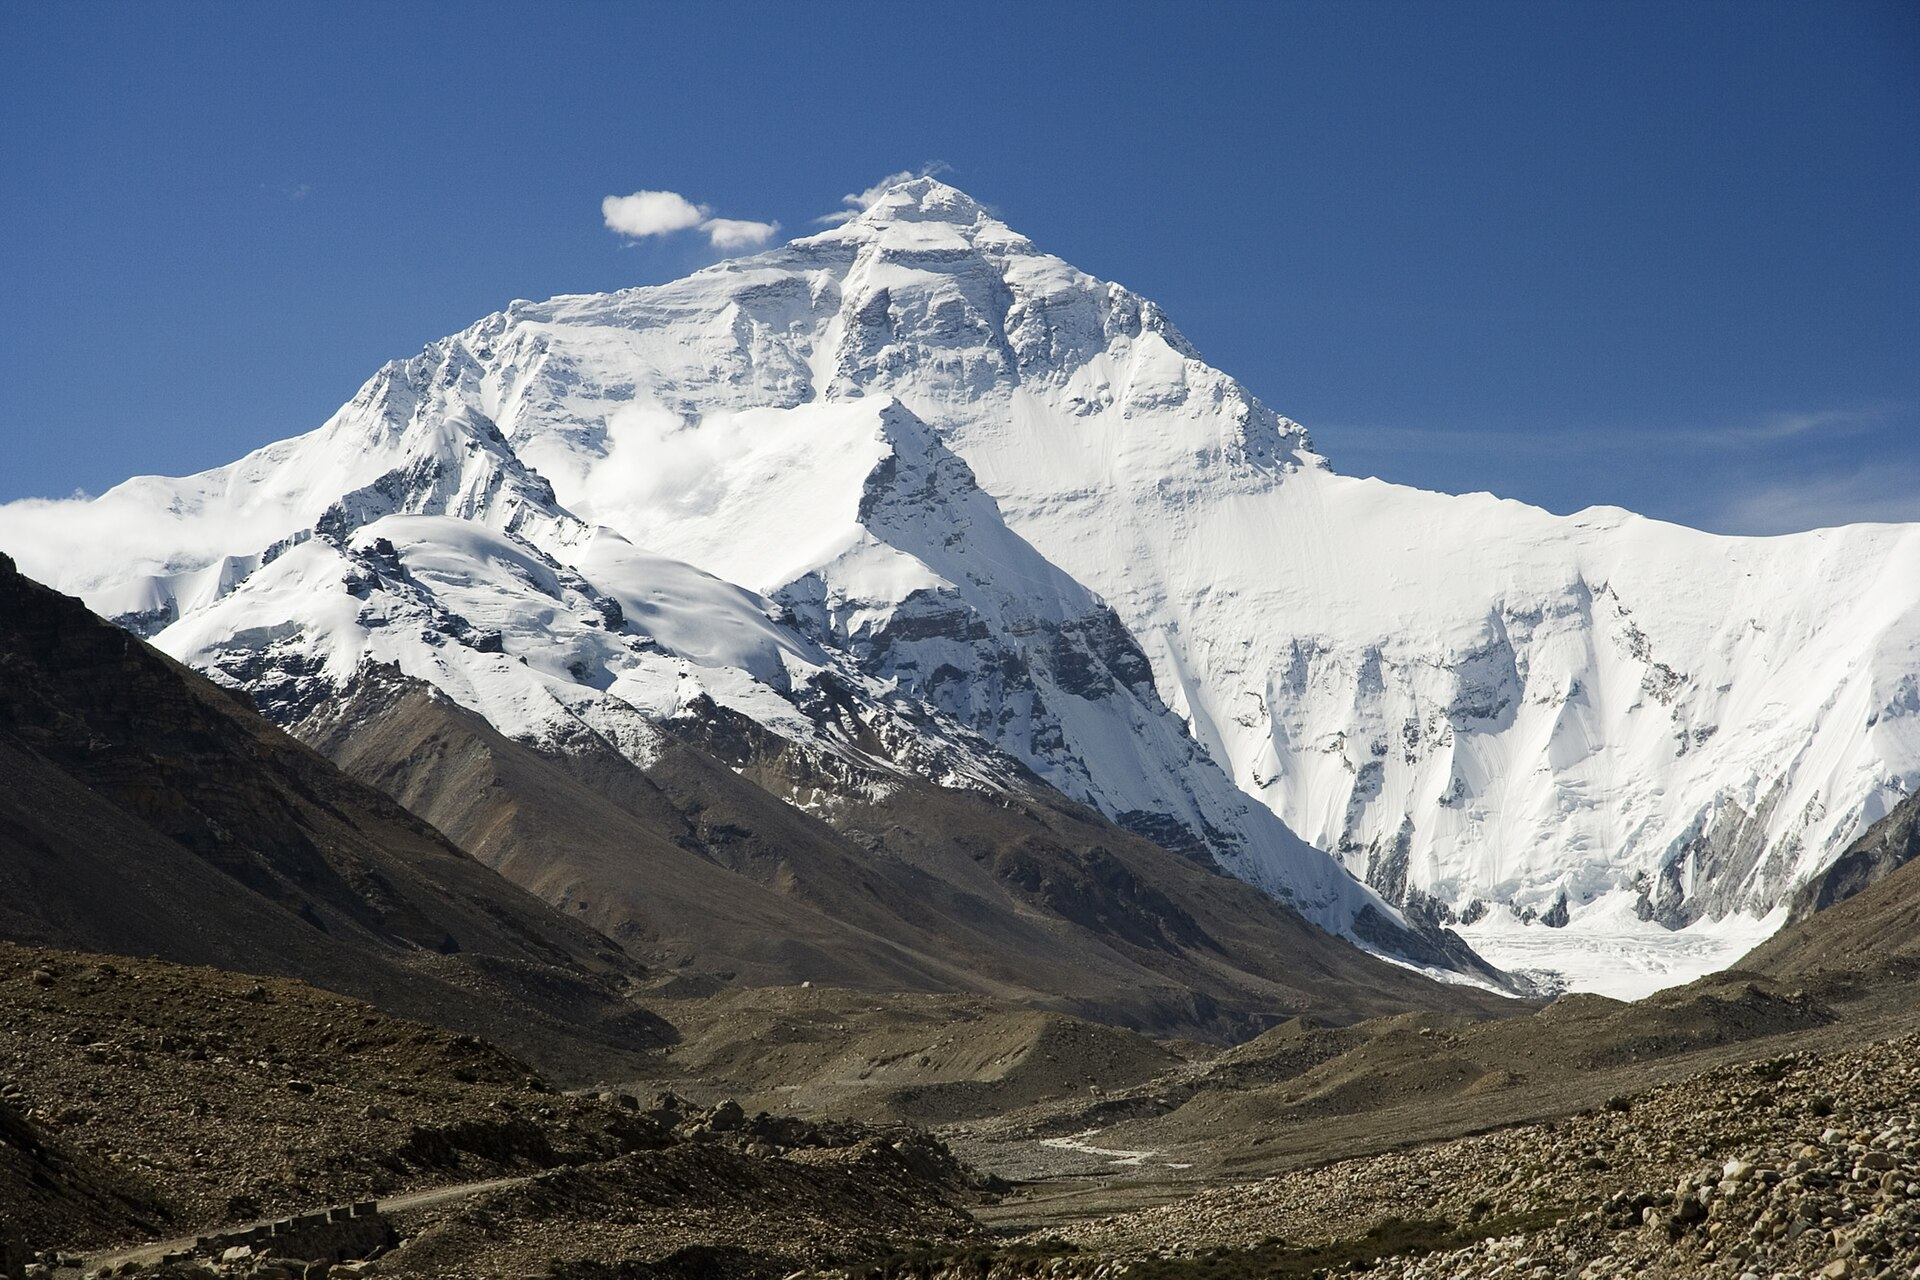
\includegraphics[height=\paperheight]{img/everest.jpg}};
  \end{scope}
  \node[anchor=west, text width=0.5\paperwidth, align=left] at ([xshift=0.06\paperwidth, yshift=0.06\paperheight]current page.west) {%
    {\LARGE\bfseries\color{navy}\hyphenpenalty=10000 How Much of Summit\\ Success Is Decided\\ Before the Climb?\par}
    \vspace{0.8em}
    {\normalsize Predicting individual summit success on Himalayan expeditions\par}
    \vspace{0.6em}
    {\color{black!25}\rule{0.46\paperwidth}{0.4pt}\par}
    \vspace{0.6em}
    {Dávid Zoltán Dócs \qquad Dávid Szaniszló\par}
    \vspace{0.6em}
    {\small Statistical and Machine Learning\par}
    {\small 17 November 2026\par}};
  \node[anchor=south west, text=black!50, font=\tiny, inner sep=0pt] at ([xshift=0.06\paperwidth, yshift=4mm]current page.south west)
    {Photo: Mount Everest, north face (L.\ Galuzzi, CC BY-SA 2.5)};
\end{tikzpicture}
\end{frame}

% ---------------------------------------------------------------- 1 (0:55)
\begin{frame}{Motivation and research question}
\begin{columns}[T]
\column{0.48\textwidth}
\textbf{Context}
\begin{itemize}\small
  \item A Himalayan expedition takes weeks and costs tens of thousands of euros
  \item About one in three climbers reaches the summit
  \item Peak, season, team and hired support are fixed months in advance
\end{itemize}
\vspace{0.6em}
\textbf{Dataset}
\begin{itemize}\small
  \item Near-complete record of expeditions in Nepal, 55,049 climbers
  \item Non-linear effects and interactions
  \item Two methodological issues: leakage and clustered observations
\end{itemize}
\column{0.48\textwidth}
\begin{block}{Research question}
\small Using only information available before departure, how well can we predict whether a climber reaches the summit, and which factors drive the probability?
\end{block}
\vspace{0.5em}
\small
Binary classification: $Y_i \in \{0,1\}$, estimate $p(x) = P(Y = 1 \mid X = x)$.
\begin{enumerate}\small
  \item How well can we predict?
  \item Which method performs best?
  \item Which factors matter?
  \item How reliable are the predictions?
\end{enumerate}
\end{columns}
\end{frame}

% ---------------------------------------------------------------- 2 (0:50)
\begin{frame}{Data}
\begin{columns}[T]
\column{0.45\textwidth}
\begin{itemize}\small
  \item Expedition archive of the Nepal Himalaya compiled by Elizabeth Hawley, 1905\textendash 2019
  \item Three tables, members (76,519), expeditions (10,364) and peaks (468), joined to one row per climber
  \item Target: \texttt{success} of the individual climber
  \item Hired staff are excluded: they reach the summit 65\% of the time, as part of their job
  \item Sample: 55,049 climbers, 9,883 expeditions, 381 peaks; summit rate 33.8\%
\end{itemize}
\column{0.5\textwidth}
\begin{table}
\footnotesize
\begin{tabular}{lr}
\toprule
Filter step & Climbers \\
\midrule
All member records & 76,519 \\
Year 1950 or later & 76,099 \\
Not hired staff & 60,533 \\
Climbing role (no doctors, film crews) & 56,443 \\
Expedition attempted the climb & 55,062 \\
Peak, sex and season known & \textbf{55,049} \\
\bottomrule
\end{tabular}
\caption{Construction of the analysis sample.}
\end{table}
\end{columns}
\end{frame}

% ---------------------------------------------------------------- 3 (1:10)
\begin{frame}{Exploratory analysis}
\fig[width=\textwidth]{fig01_eda.png}{Summit rate by year, peak, season, age and hired staff per climber. Dashed: overall rate (34\%).}
\end{frame}

% ---------------------------------------------------------------- 4 (1:00)
\begin{frame}{Pre-processing}
\begin{columns}[T]
\column{0.46\textwidth}
\textbf{Predictors (16)}
\begin{itemize}\small
  \item Mountain: peak (top 10 + other), height, 8000\,m peak, climbed before
  \item Time: year, season
  \item Team and support: hired staff, staff per climber, commercial agency, team size, solo
  \item Climber: age (median imputation + missing indicator), sex, citizenship (top 15 + other), leader
\end{itemize}
\vspace{0.4em}
\textbf{Excluded as leakage}
\begin{itemize}\small
  \item highest point reached, death, injury, termination reason
  \item oxygen use: recorded high on the mountain, so it reveals how far the climber got (Figure~\ref{fig:oxygen})
\end{itemize}
\column{0.5\textwidth}
\begin{figure}
\centering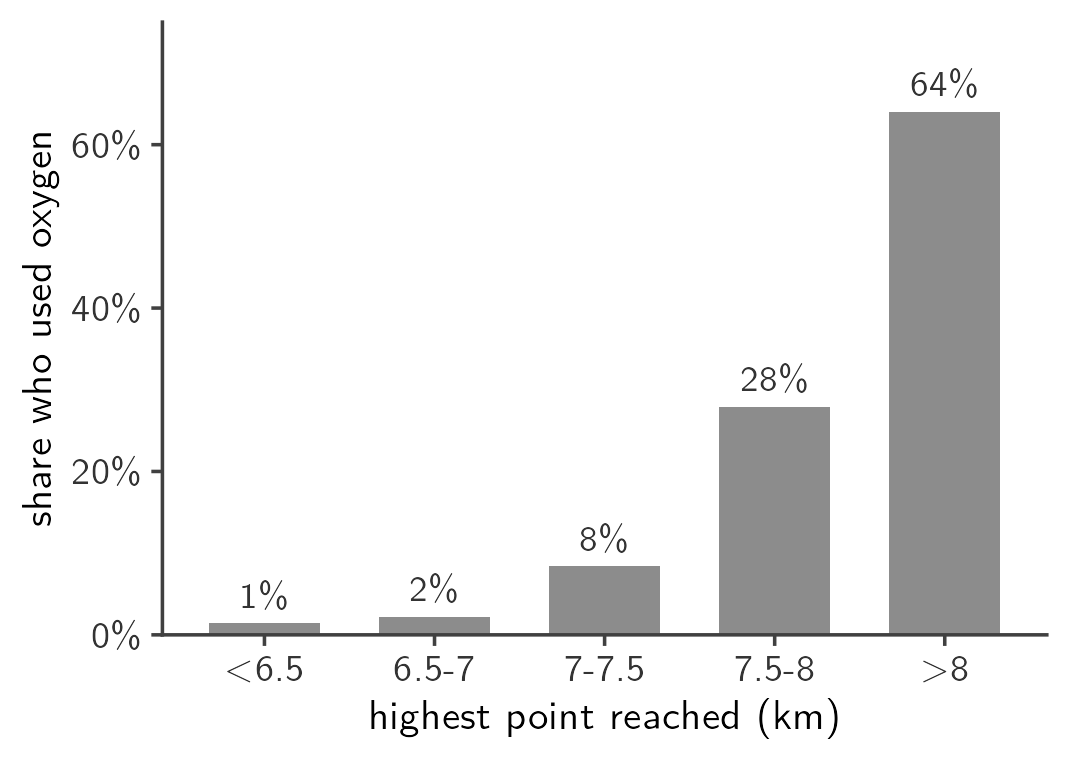
\includegraphics[width=2.7in]{fig03_oxygen_leakage.png}
\caption{Oxygen use among climbers who failed on 8000\,m peaks, by highest point reached.}
\label{fig:oxygen}
\end{figure}
\end{columns}
\end{frame}

% ---------------------------------------------------------------- 5 (1:10)
\begin{frame}{Validation design and evaluation metrics}
\begin{columns}[T]
\column{0.44\textwidth}
\begin{figure}
\centering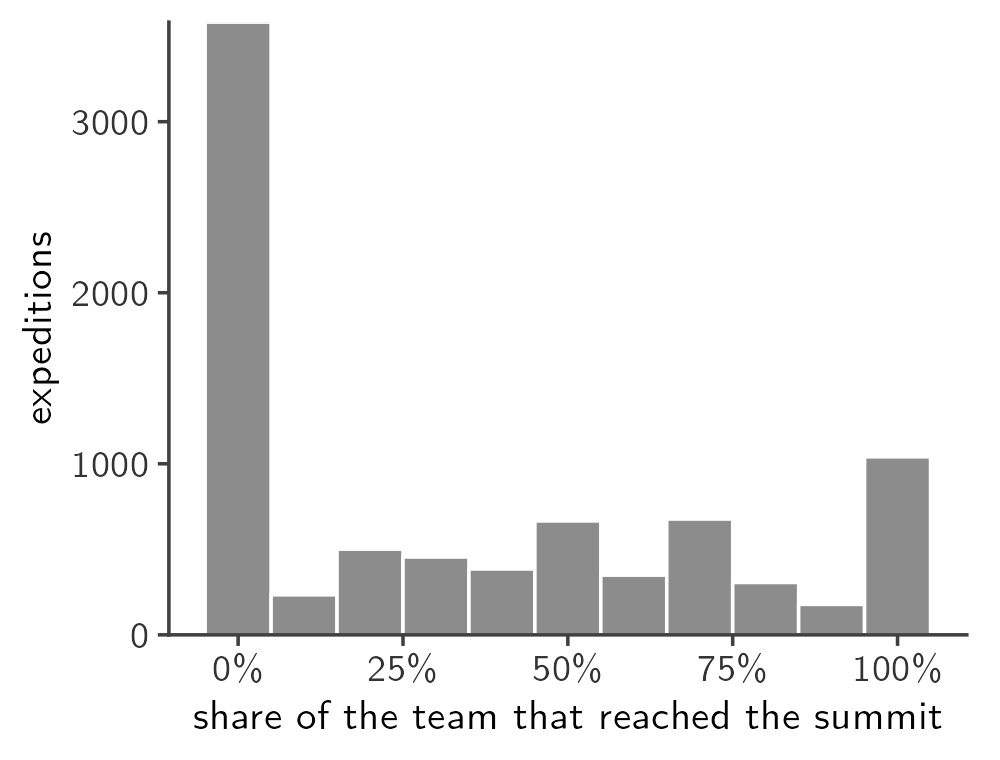
\includegraphics[width=2.5in]{fig04_clustering.png}
\caption{Share of the team reaching the summit, per expedition.}
\label{fig:cluster}
\end{figure}
\column{0.53\textwidth}
\textbf{Sample splitting}
\begin{itemize}\footnotesize
  \item Outcomes are clustered within expeditions (Figure~\ref{fig:cluster}): in 43\% nobody summits, in 12\% everybody does
  \item Test set: 20\% of \emph{expeditions} (11,133 climbers), used once
  \item Tuning: 5-fold CV with folds formed by expedition
  \item Imputation and category grouping estimated on the training set
\end{itemize}
\vspace{0.4em}
\textbf{Metrics}
\begin{itemize}\footnotesize
  \item Log score (main) and Brier score, both strictly proper:
  \vspace{-0.3em}
  \begin{align*}
  \mathrm{LS} &= \textstyle -\frac{1}{N}\sum_{i} \bigl[y_i \log \hat p_i + (1-y_i)\log(1-\hat p_i)\bigr]\\[-0.2em]
  \mathrm{BS} &= \textstyle \frac{1}{N}\sum_{i} (\hat p_i - y_i)^2
  \end{align*}
  \vspace{-1.2em}
  \item AUC for discrimination, calibration plots
  \item Accuracy is of limited use: predicting ``no summit'' for everyone gives 68\%
\end{itemize}
\end{columns}
\end{frame}

% ---------------------------------------------------------------- 6 (1:10)
\begin{frame}{Methods}
\begin{table}
\footnotesize
\renewcommand{\arraystretch}{1.4}
\begin{tabular}{@{}>{\raggedright}p{0.15\textwidth}>{\raggedright}p{0.37\textwidth}>{\raggedright}p{0.21\textwidth}>{\raggedright\arraybackslash}p{0.19\textwidth}@{}}
\toprule
Method & Model / objective & Tuning (grouped 5-fold CV) & Selected \\
\midrule
Elastic-net logistic regression &
  $\min_\beta\, -\frac{1}{N}\ell(\beta) + \lambda\bigl[\frac{1-\alpha}{2}\|\beta\|_2^2 + \alpha\|\beta\|_1\bigr]$; natural splines for year, age and height &
  $\alpha \in \{0, .25, .5, .75, 1\}$, $\lambda$ path, 1-SE rule & $\alpha = 0.25$, 38 of 49 terms \\
Classification tree &
  Cost-complexity pruning, $C_{cp}(T) = R(T) + cp\,|T|$ &
  $cp$, 1-SE rule & 30 leaves \\
Random forest &
  Average of $B = 500$ trees grown on bootstrap samples, $m$ of 16 predictors tried at each split &
  $m \in \{2,4,7,11\}$ $\times$ minimum node size $\in \{25, 100, 400, 1000\}$ & $m = 7$, node size 100 \\
Gradient boosting &
  $f_M(x) = f_{M-1}(x) + \nu\, T(x; \Theta_M)$, Bernoulli deviance &
  depth $J \times$ shrinkage $\nu \times$ trees $M$ & $J = 6$, $\nu = 0.02$, $M = 2{,}850$ \\
\bottomrule
\end{tabular}
\caption{Methods, tuning grids and selected values (training set only).}
\end{table}
\end{frame}

% ---------------------------------------------------------------- 7 (1:00)
\begin{frame}{Tuning}
\begin{columns}[T]
\column{0.66\textwidth}
\fig[width=3.65in]{fig06_tuning.png}{Grouped 5-fold CV error. Vertical lines: 1-SE choice; circle: selected setting.}
\column{0.31\textwidth}
\vspace{0.4em}
\begin{itemize}\small
  \item Elastic net: $\alpha$ hardly matters; 38 of 49 terms kept
  \item Tree: 30 leaves
  \item Forest: out-of-bag error (dashed) too optimistic, 0.50 vs.\ 0.57, since team-mates stay in the bootstrap sample
  \item Boosting: deepest trees ($J = 6$) win, so interactions matter
\end{itemize}
\end{columns}
\end{frame}

% ---------------------------------------------------------------- 8 (1:10)
\begin{frame}{Model assessment on the test set}
\begin{columns}[T]
\column{0.53\textwidth}
\cell{table}{1.95in}{\footnotesize
\begin{tabular}{lcccc}
\toprule
Model & Log loss & Brier & AUC & Accuracy \\
\midrule
Summit rate only & 0.629 & 0.219 & 0.500 & 0.678 \\
Elastic net      & 0.582 & 0.198 & 0.695 & 0.697 \\
Pruned tree      & 0.579 & 0.196 & 0.685 & 0.716 \\
Random forest    & 0.543 & 0.181 & 0.748 & 0.736 \\
\textbf{Boosting} & \textbf{0.533} & \textbf{0.178} & \textbf{0.757} & \textbf{0.738} \\
\bottomrule
\end{tabular}}{Test-set performance (11,133 climbers).}
\column{0.43\textwidth}
\cell{figure}{1.95in}{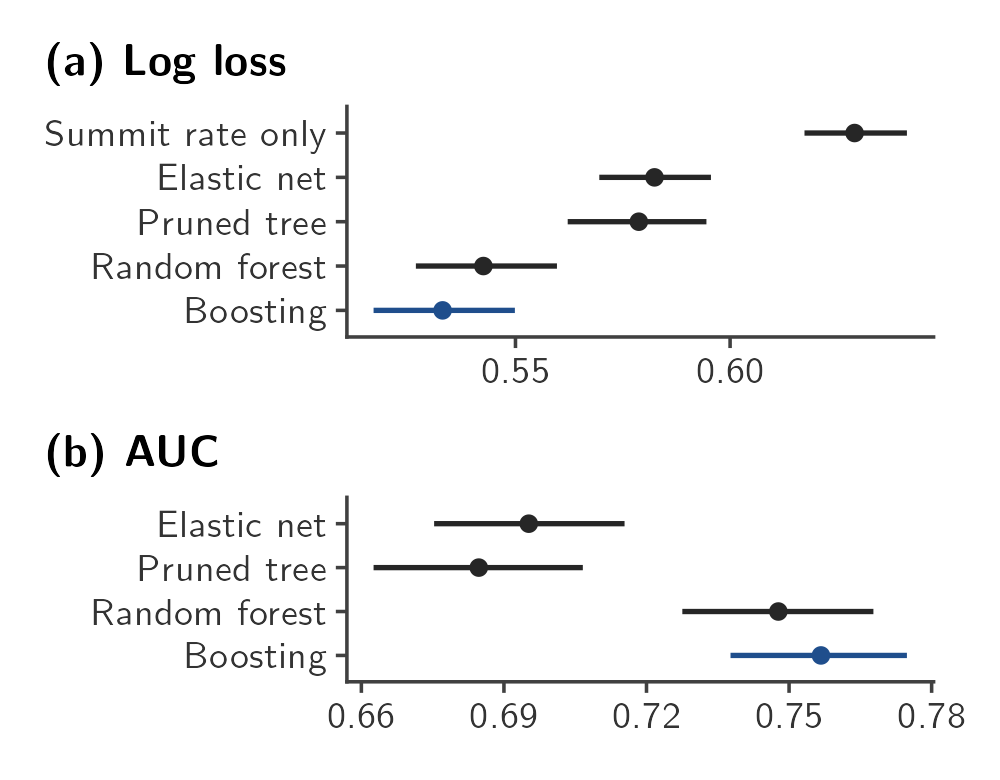
\includegraphics[width=2.5in]{fig07_comparison.png}}{Test metrics with 95\% bootstrap intervals.}
\end{columns}
\vspace{0.2em}
\begin{itemize}\small
  \item Random forest and boosting clearly outperform the elastic net and the single tree
  \item Boosting vs.\ random forest: difference in log loss 0.010, 95\% CI $[0.003, 0.016]$
\end{itemize}
\end{frame}

% ---------------------------------------------------------------- 9 (1:00)
\begin{frame}{ROC curves and confusion matrix}
\begin{columns}[T]
\column{0.6\textwidth}
\cell{figure}{2.0in}{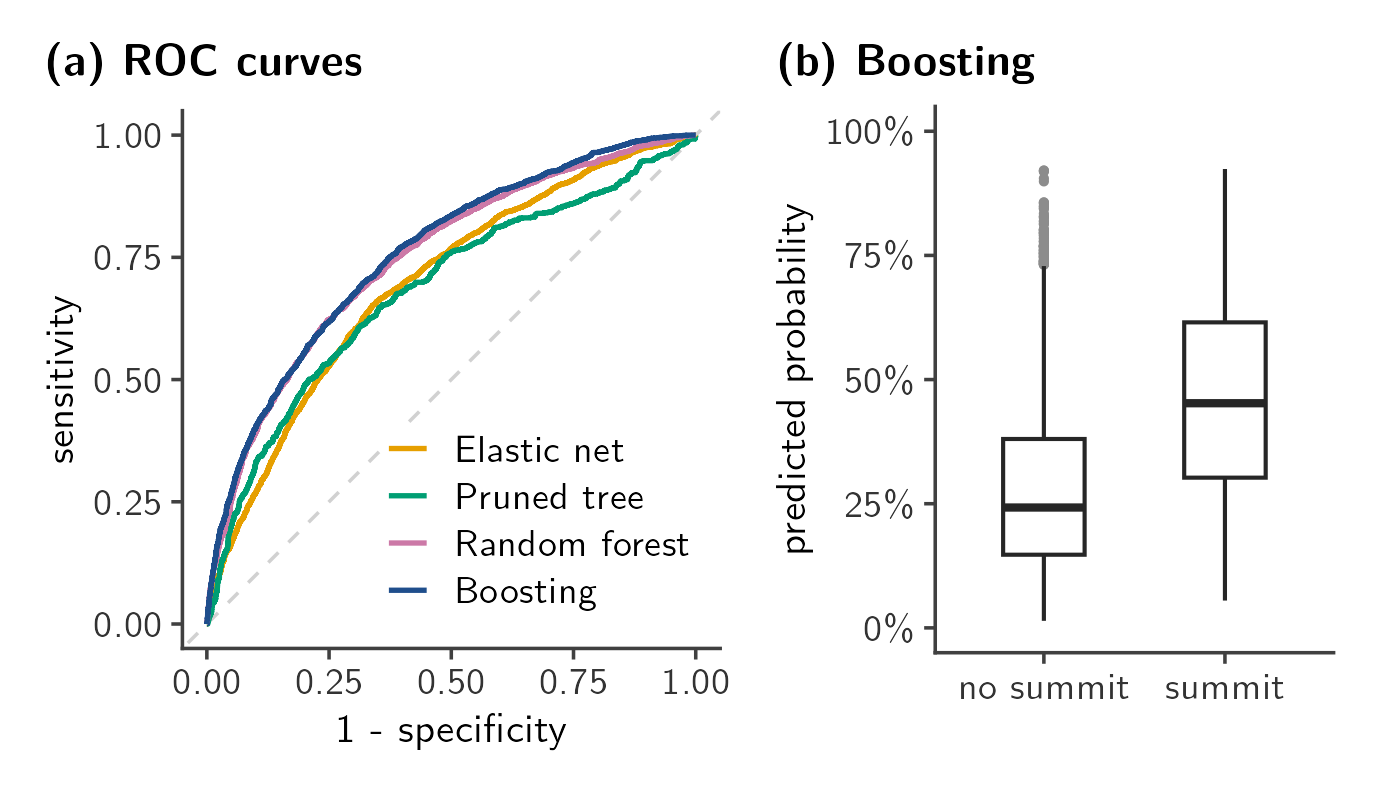
\includegraphics[width=3.5in]{fig17_discrimination.png}}{(a) ROC curves. (b) Boosting predictions by observed outcome.}
\column{0.37\textwidth}
\cell{table}{2.0in}{\footnotesize
\begin{tabular}{lcc}
\toprule
 & \multicolumn{2}{c}{Observed} \\
Predicted & Summit & No summit \\
\midrule
Summit    & 1,531 & 863 \\
No summit & 2,050 & 6,689 \\
\bottomrule
\end{tabular}}{Boosting confusion matrix, cut-off 0.5.}
\end{columns}
\vspace{0.2em}
\begin{columns}[T]
\column{0.48\textwidth}
\begin{itemize}\small
  \item Sensitivity 0.43, specificity 0.89
  \item Precision 0.64
\end{itemize}
\column{0.48\textwidth}
\begin{itemize}\small
  \item Cut-off at the summit rate (0.34): sensitivity and specificity both 0.69
\end{itemize}
\end{columns}
\end{frame}

% ---------------------------------------------------------------- 10 (1:00)
\begin{frame}{Predicted and observed summit rates}
\begin{columns}[T]
\column{0.6\textwidth}
\fig[width=3.5in]{fig09_deciles.png}{Observed (bars) and predicted (dots) summit rate by decile of the boosting prediction.}
\column{0.37\textwidth}
\begin{itemize}\small
  \item Without a model, every climber gets 34\%
  \item The model separates test climbers into groups with 6\% to 73\% observed success
  \item Predicted and observed rates agree in every decile, so the model is well calibrated
  \item Log loss is 15\% below the baseline; much of the outcome remains unexplained
\end{itemize}
\end{columns}
\end{frame}

% ---------------------------------------------------------------- 11 (1:00)
\begin{frame}{Interpretable models: logit coefficients and pruned tree}
\begin{columns}[T]
\column{0.42\textwidth}
\cell{table}{2.1in}{\footnotesize
\begin{tabular}{lrc}
\toprule
Term & $\hat\beta$ & Odds ratio \\
\midrule
log(1 + staff per climber) & 0.58 & 1.79 \\
Peak: Cho Oyu            & 0.40 & 1.50 \\
Peak: Annapurna I        & $-0.36$ & 0.70 \\
Peak: Everest            & $-0.26$ & 0.77 \\
Season: winter           & $-0.16$ & 0.85 \\
Role: leader             & 0.15 & 1.16 \\
Citizenship: China       & 0.56 & 1.75 \\
Citizenship: South Korea & $-0.42$ & 0.66 \\
\bottomrule
\end{tabular}}{Elastic net at $\lambda_{1\text{-SE}}$. Reference: autumn, other peaks, climber, other citizenship.}
\column{0.54\textwidth}
\cell{figure}{2.1in}{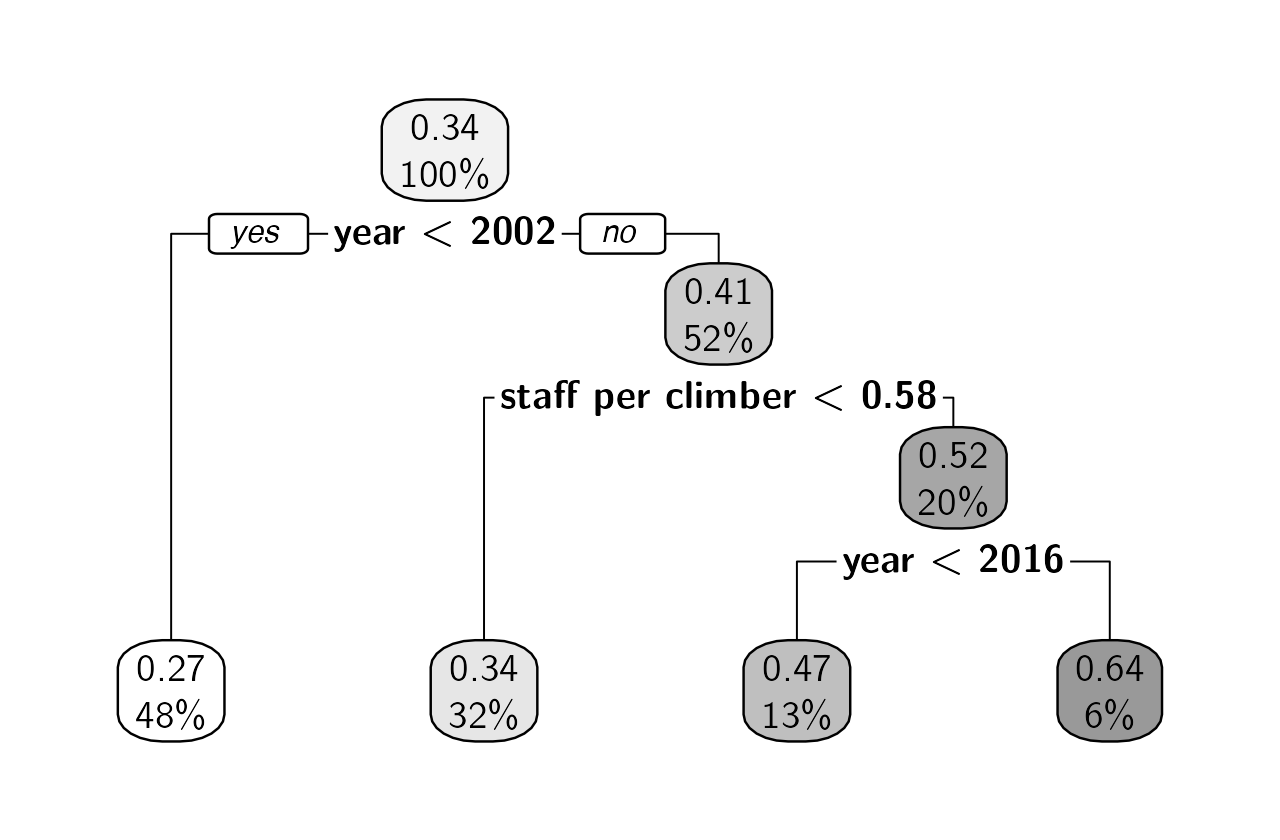
\includegraphics[width=3.2in]{fig12_tree.png}}{Pruned tree, first splits. Nodes: summit rate and share of climbers.}
\end{columns}
\end{frame}

% ---------------------------------------------------------------- 12 (1:10)
\begin{frame}{Boosting: importance and partial dependence}
\begin{columns}[T]
\column{0.37\textwidth}
\cell{figure}{2.45in}{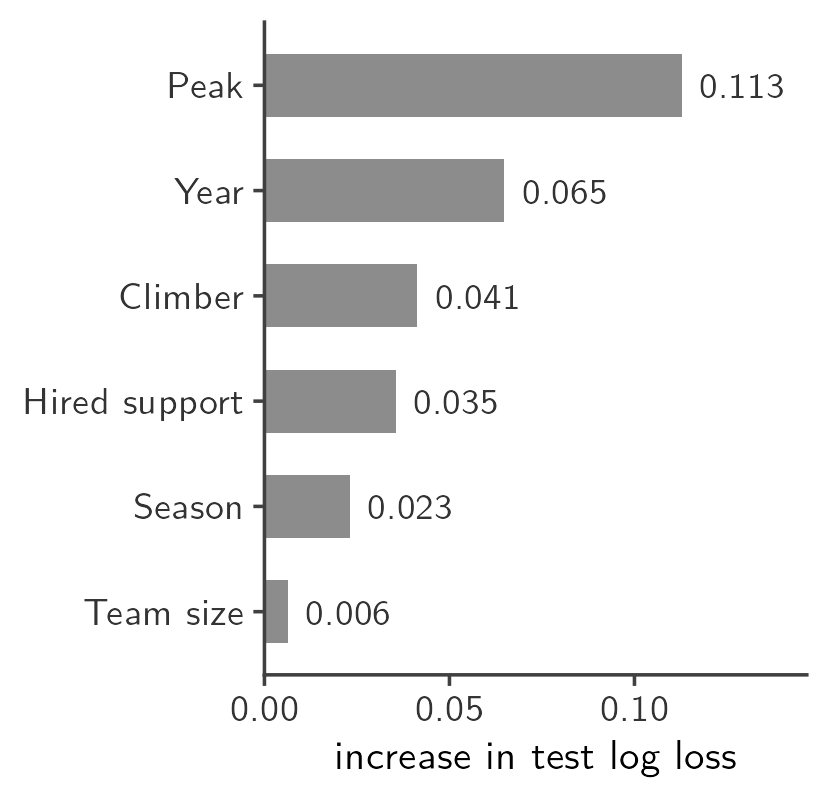
\includegraphics[width=2.1in]{fig10_importance.png}}{Permutation importance by group of predictors.}
\column{0.6\textwidth}
\cell{figure}{2.45in}{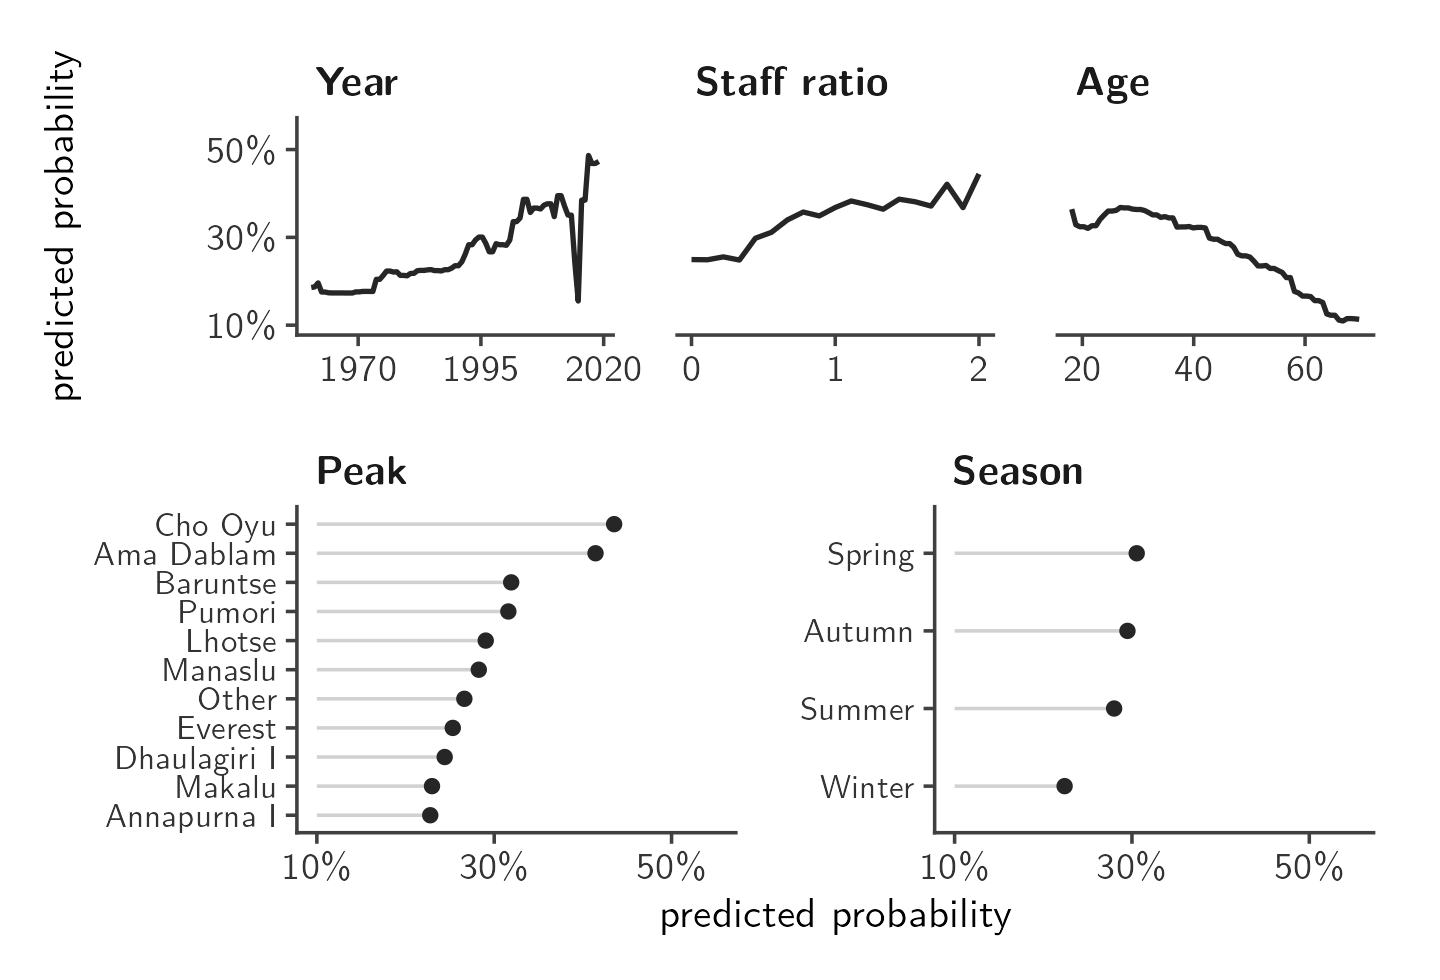
\includegraphics[width=3.6in]{fig11_partial_dependence.png}}{Partial dependence of the boosting prediction (dip in 2015: earthquake).}
\end{columns}
\end{frame}

% ---------------------------------------------------------------- 13 (1:15)
\begin{frame}{Robustness checks}
\begin{columns}[T]
\column{0.48\textwidth}
\cell{figure}{1.6in}{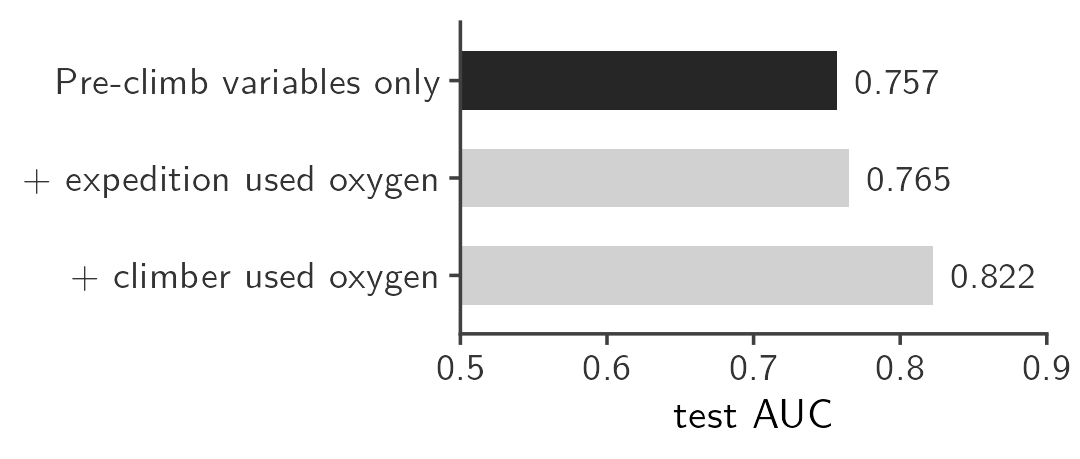
\includegraphics[width=2.7in]{fig15_leakage.png}}{Boosting test AUC with oxygen variables added.}
\begin{itemize}\small
  \item Adding oxygen use raises the AUC from 0.76 to 0.82
  \item The gain comes from information recorded during the climb, so it is not available before departure
\end{itemize}
\column{0.48\textwidth}
\cell{figure}{1.6in}{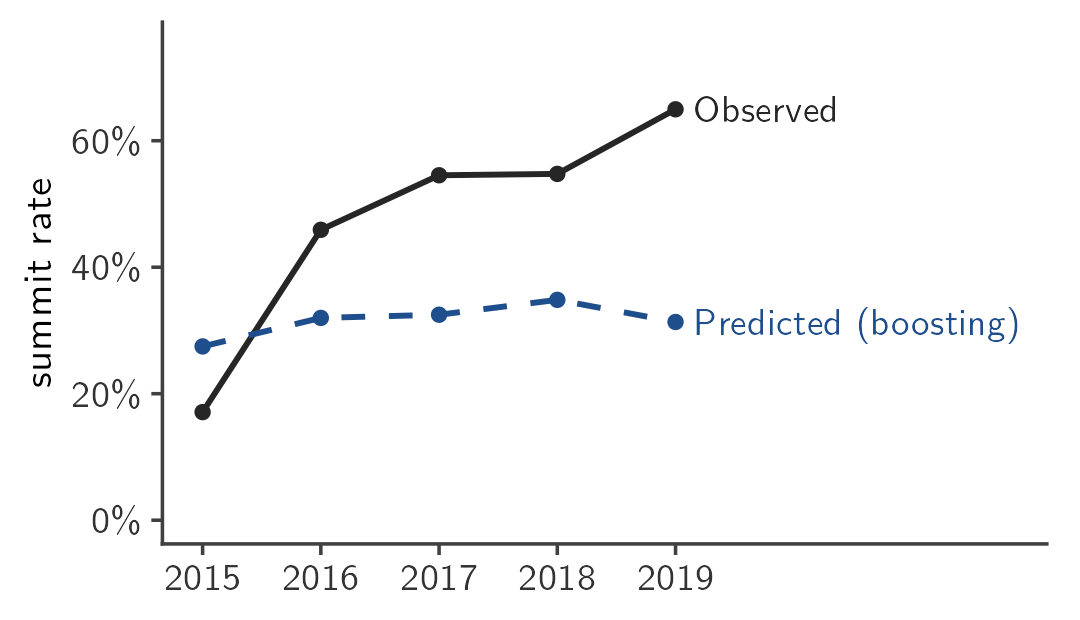
\includegraphics[width=2.7in]{fig16_time_split.png}}{Trained on 1950\textendash 2014, predicted for 2015\textendash 2019.}
\begin{itemize}\small
  \item The ranking still works (AUC 0.63\textendash 0.66)
  \item The level is too low (32\% vs.\ 47\%)
  \item Trees cannot extrapolate the trend, so the model needs refitting for new seasons
\end{itemize}
\end{columns}
\end{frame}

% ---------------------------------------------------------------- 14 (1:00)
\begin{frame}{Conclusion and limitations}
\begin{columns}[T]
\column{0.55\textwidth}
\textbf{Findings}
\begin{enumerate}\small
  \item Pre-climb information separates climbers into groups with 6\% to 73\% success; boosting reaches an AUC of 0.76 and is well calibrated
  \item Boosting $>$ random forest $>$ tree $\approx$ elastic net; the gain of the flexible models indicates non-linear effects and interactions
  \item Peak and year matter most, followed by age, citizenship and hired support
  \item Grouped validation and the removal of leaky variables change the results (OOB 0.50 vs.\ CV 0.57; leaky AUC 0.82)
\end{enumerate}
\column{0.4\textwidth}
\textbf{Limitations}
\begin{itemize}\small
  \item No data on weather, health or experience of the climber
  \item Strong changes over time limit forecasts for new seasons
  \item Associations only, no causal effects
  \item Nepal only, data up to spring 2019
\end{itemize}
\end{columns}
\end{frame}

\begin{frame}{References}
\scriptsize
\setlength{\parskip}{0.4em}
Breiman, L. (2001). Random forests. \textit{Machine Learning} 45, 5\textendash 32.

Friedman, J. (2001). Greedy function approximation: a gradient boosting machine. \textit{Annals of Statistics} 29(5), 1189\textendash 1232.

Friedman, J., Hastie, T. and Tibshirani, R. (2010). Regularization paths for generalized linear models via coordinate descent. \textit{Journal of Statistical Software} 33(1).

Hastie, T., Tibshirani, R. and Friedman, J. (2009). \textit{The Elements of Statistical Learning}, 2nd ed. Springer.

Hawley, E. and Salisbury, R. \textit{The Himalayan Database}. himalayandatabase.com

James, G., Witten, D., Hastie, T. and Tibshirani, R. (2021). \textit{An Introduction to Statistical Learning}, 2nd ed. Springer.

Mock, T. (2020). TidyTuesday 2020-09-22: Himalayan climbing expeditions. github.com/rfordatascience/tidytuesday

Ridgeway, G. and GBM Developers. \texttt{gbm}: Generalized boosted regression models. R package.

Therneau, T. and Atkinson, B. \texttt{rpart}: Recursive partitioning and regression trees. R package.

Wright, M. N. and Ziegler, A. (2017). \texttt{ranger}: A fast implementation of random forests. \textit{Journal of Statistical Software} 77(1).

Title photo: Galuzzi, L. (2006). \textit{Everest North Face toward Base Camp, Tibet}. Wikimedia Commons, CC BY-SA 2.5.
\end{frame}

\begin{frame}
\vfill
\centering
{\Large\bfseries\color{navy} Thank you!\par}
\vfill
\end{frame}

% ================================================================ BACKUP
\appendix
\begin{frame}
\vfill
\centering
{\Large\bfseries\color{navy} Backup\par}
\vfill
\end{frame}

\begin{frame}{Backup: test results with 95\% bootstrap intervals}
\begin{table}
\small
\begin{tabular}{lcc}
\toprule
Model & Log loss & AUC \\
\midrule
Summit rate only & 0.629 \;[0.617, 0.641] & 0.500 \\
Elastic net      & 0.582 \;[0.570, 0.596] & 0.695 \;[0.675, 0.715] \\
Pruned tree      & 0.579 \;[0.562, 0.594] & 0.685 \;[0.663, 0.707] \\
Random forest    & 0.543 \;[0.527, 0.560] & 0.748 \;[0.728, 0.768] \\
\textbf{Boosting} & \textbf{0.533} \;[0.517, 0.550] & \textbf{0.757} \;[0.738, 0.775] \\
\bottomrule
\end{tabular}
\caption{Test metrics with 95\% intervals (1,000 bootstrap samples of test expeditions).}
\end{table}
\small Training set: 43,916 climbers from 7,906 expeditions. Log-loss advantage of boosting: 0.010 over the random forest [0.003, 0.016], 0.046 over the tree [0.035, 0.056], 0.049 over the elastic net [0.039, 0.060]. No interval contains zero.
\end{frame}

\begin{frame}{Backup: confusion matrices of all models}
\begin{table}
\footnotesize
\begin{tabular}{lccccccc}
\toprule
Model & Cut-off & TP & FN & FP & TN & Sensitivity & Specificity \\
\midrule
Elastic net   & 0.50 & 546   & 3,035 & 336   & 7,216 & 0.15 & 0.96 \\
Pruned tree   & 0.50 & 1,223 & 2,358 & 803   & 6,749 & 0.34 & 0.89 \\
Random forest & 0.50 & 1,359 & 2,222 & 713   & 6,839 & 0.38 & 0.91 \\
Boosting      & 0.50 & 1,531 & 2,050 & 863   & 6,689 & 0.43 & 0.89 \\
Boosting      & 0.34 & 2,457 & 1,124 & 2,347 & 5,205 & 0.69 & 0.69 \\
\bottomrule
\end{tabular}
\caption{Test-set confusion matrices; positive class: summit reached.}
\end{table}
\small 3,581 of 11,133 test climbers reached the summit. A cut-off of 0.5 favours specificity because only a third of the climbers summit. The cut-off can be set by the cost of each error; log loss and Brier score do not depend on it.
\end{frame}

\begin{frame}{Backup: calibration of all four models}
\fig[width=\textwidth]{fig08_calibration.png}{Observed vs.\ predicted summit rate by decile (test set). Dashed: perfect calibration.}
\small All models lie close to the diagonal. The elastic net and the tree spread their predictions less (20\% to 60\%); random forest and boosting range from below 10\% to above 70\%.
\end{frame}

\begin{frame}{Backup: elastic-net coefficient paths}
\fig[width=3.1in]{fig18_en_path.png}{Coefficient paths. Dashed: $\lambda_{1\text{-SE}}$; dotted: $\lambda_{\min}$.}
\begin{itemize}\small
  \item CV deviance is 1.193 for every $\alpha > 0$ and 1.195 for ridge, so the choice of $\alpha$ hardly matters
  \item The tree reaches its minimum CV error at 64 leaves; the 1-SE rule gives 30
\end{itemize}
\end{frame}

\begin{frame}{Backup: tuning grids}
\begin{columns}[T]
\column{0.48\textwidth}
\cell{table}{1.35in}{\footnotesize
\begin{tabular}{cccc}
\toprule
$m$ & Node size & CV log loss & OOB \\
\midrule
\textbf{7} & \textbf{100} & \textbf{0.567} & 0.499 \\
4 & 100 & 0.568 & 0.508 \\
4 & 25 & 0.569 & 0.475 \\
11 & 100 & 0.569 & 0.497 \\
7 & 25 & 0.572 & 0.467 \\
11 & 25 & 0.576 & 0.467 \\
2 & 1000 & 0.590 & 0.578 \\
\bottomrule
\end{tabular}}{Random forest (selected rows of the $4 \times 4$ grid).}
\column{0.48\textwidth}
\cell{table}{1.35in}{\footnotesize
\begin{tabular}{cccc}
\toprule
Depth $J$ & Shrinkage $\nu$ & Trees $M$ & CV log loss \\
\midrule
\textbf{6} & \textbf{0.02} & \textbf{2,850} & \textbf{0.562} \\
4 & 0.02 & 2,950 & 0.564 \\
6 & 0.1 & 350 & 0.565 \\
4 & 0.1 & 1,000 & 0.567 \\
2 & 0.1 & 1,100 & 0.572 \\
2 & 0.02 & 3,000 & 0.572 \\
\bottomrule
\end{tabular}}{Gradient boosting, best number of trees per setting.}
\end{columns}
\small Both tuned by grouped 5-fold CV. OOB would select the smallest node size.
\end{frame}

\begin{frame}{Backup: variable importance}
\begin{columns}[T]
\column{0.48\textwidth}
\fig[width=2.75in]{fig13_importance_rf.png}{Random forest. Gini overrates age (0.43 vs.\ 0.17).}
\column{0.48\textwidth}
\fig[width=2.75in]{fig19_importance_gbm.png}{Boosting. Relative influence overrates citizenship.}
\end{columns}
\end{frame}

\begin{frame}{Backup: one climber, different plans}
\fig[width=\textwidth]{fig14_plans.png}{Boosting predictions for a 40-year-old US climber in 2019 under different plans.}
\small These are model predictions, not causal effects: climbers who go without hired staff also differ in other respects.
\end{frame}

\begin{frame}{Backup: time split, all models}
\begin{table}
\small
\begin{tabular}{lccc}
\toprule
Model & Log loss & AUC & Mean predicted \\
\midrule
Summit rate only & 0.740 & 0.500 & 32\% \\
Elastic net      & 0.703 & 0.627 & 34\% \\
Pruned tree      & 0.668 & 0.648 & 42\% \\
Random forest    & 0.692 & 0.638 & 34\% \\
Boosting         & 0.713 & 0.661 & 32\% \\
\midrule
Observed         &       &       & 47\% \\
\bottomrule
\end{tabular}
\caption{Trained on 1950\textendash 2014, evaluated on 2015\textendash 2019 (7,258 climbers).}
\end{table}
\small Boosting ranks future climbers best (highest AUC) but has a worse log loss than the tree, because all models underestimate the higher summit rates after 2015. The main test set measures performance on new expeditions from the same period.
\end{frame}

\begin{frame}{Backup: random vs.\ grouped cross-validation}
\begin{table}
\footnotesize
\begin{tabular}{lcccccc}
\toprule
 & \multicolumn{2}{c}{Random 5-fold CV} & \multicolumn{2}{c}{Grouped 5-fold CV} & \multicolumn{2}{c}{Test set} \\
Model & Log loss & AUC & Log loss & AUC & Log loss & AUC \\
\midrule
Random forest & 0.508 & 0.807 & 0.568 & 0.727 & 0.543 & 0.748 \\
Boosting      & 0.519 & 0.789 & 0.562 & 0.735 & 0.533 & 0.757 \\
\bottomrule
\end{tabular}
\caption{Same tuned settings, folds formed at random (climbers) or by expedition.}
\end{table}
\begin{itemize}\small
  \item Random folds put team-mates on both sides and make the models look 0.04\textendash 0.06 better in log loss
  \item The test set is one 20\% draw of expeditions and somewhat easier: summit rate 32.2\% vs.\ 34.2\%, baseline log loss 0.629 vs.\ 0.643
  \item Relative to its baseline, boosting improves the log loss by 12.5\% in grouped CV and by 15\% on the test set
\end{itemize}
\end{frame}

\begin{frame}{Backup: does the penalty help?}
\begin{table}
\footnotesize
\begin{tabular}{lccc}
\toprule
Model (same 49 terms) & Non-zero terms & Test log loss & Test AUC \\
\midrule
Logistic regression, no penalty & 49 & 0.575 & 0.701 \\
Elastic net, $\lambda_{\min}$   & 48 & 0.575 & 0.701 \\
Elastic net, $\lambda_{1\text{-SE}}$ (used) & 38 & 0.582 & 0.695 \\
\bottomrule
\end{tabular}
\caption{Linear models on the test set.}
\end{table}
\begin{itemize}\small
  \item With 55,049 climbers and 49 terms the penalty adds little: $\lambda_{\min}$ equals the unpenalised fit
  \item The 1-SE rule gives up 0.007 in log loss for 11 fewer terms
  \item Random forest and boosting are 0.03\textendash 0.04 better than every linear version, so the conclusions do not change
\end{itemize}
\end{frame}

\begin{frame}{Backup: is hired staff only a proxy for era or commercial expeditions?}
\fig[width=\textwidth]{fig20_staff.png}{Staff per climber over time and summit rate by staff per climber since 2000. Groups with fewer than 50 climbers omitted.}
\vspace{-0.3em}
\begin{itemize}\footnotesize
  \item 82\% of climbers are on commercial expeditions; staff per climber has risen since the late 1990s
  \item Within commercial expeditions since 2000, the summit rate still rises with staff: 32\% (none) to 54\% (more than one per climber)
  \item Staff carries information beyond era and commercial status, but this remains an association
\end{itemize}
\end{frame}

\begin{frame}{Backup: why no neural network?}
\begin{itemize}
  \item The brief asks for at least three course methods; we use four, from linear to boosting
  \item The data are tabular with 16 mostly categorical predictors, where tree ensembles are usually the strongest learners
  \item Boosting with $J = 6$ already captures non-linear effects and interactions
  \item A neural network needs input scaling, dummy encoding and many more tuning choices (hidden units, weight decay, epochs), and is harder to interpret
  \item Possible extension: a single-hidden-layer network (\texttt{nnet}) tuned by the same grouped CV
\end{itemize}
\end{frame}

\begin{frame}{Backup: variable definitions}
\begin{table}
\scriptsize
\renewcommand{\arraystretch}{1.15}
\begin{tabular}{p{0.24\textwidth}p{0.66\textwidth}}
\toprule
Variable & Definition \\
\midrule
Success (target) & Climber reached the main summit \\
Year, season & Year and season of the expedition (spring, summer, autumn, winter) \\
Peak, height & Peak (10 most climbed + other) and its height in metres; 8000\,m peak indicator \\
Climbed before & Peak had a recorded first ascent before the expedition (93\% of climbers) \\
Team size & Non-hired members of the expedition \\
Hired staff & Hired staff above base camp; staff per climber = hired staff / team size \\
Commercial & Expedition organised through a trekking agency (82\% of climbers) \\
Solo & Climber listed as solo (117 climbers) \\
Age, sex, citizenship, leader & Age (2.6\% missing), sex, citizenship (15 most common + other), leader role \\
\bottomrule
\end{tabular}
\caption{The 16 predictors. All are known before departure.}
\end{table}
\end{frame}

\begin{frame}{Backup: data problems and their handling}
\begin{table}
\footnotesize
\begin{tabular}{p{0.4\textwidth}p{0.5\textwidth}}
\toprule
Problem & Handling \\
\midrule
Expedition id KANG10101 used twice (1910, 2010) & Join expeditions on id and year \\
First ascent year ``201'' & Set to missing \\
Age missing (1,417 climbers, 2.6\%) & Training median + missing indicator \\
213 citizenships, 381 peaks & Top 15 / top 10 by training frequency, rest ``other'' \\
525 role names & Keep climbing roles; climber vs.\ leader \\
Team size and hired staff strongly skewed & $\log(1+x)$ in the linear model; no transformation for trees \\
Members who never attempted the climb & Removed from the sample \\
\bottomrule
\end{tabular}
\caption{Data quality issues found in the exploratory analysis.}
\end{table}
\end{frame}

\end{document}
